\documentclass[]{book}
\usepackage{lmodern}
\usepackage{amssymb,amsmath}
\usepackage{ifxetex,ifluatex}
\usepackage{fixltx2e} % provides \textsubscript
\ifnum 0\ifxetex 1\fi\ifluatex 1\fi=0 % if pdftex
  \usepackage[T1]{fontenc}
  \usepackage[utf8]{inputenc}
\else % if luatex or xelatex
  \ifxetex
    \usepackage{mathspec}
  \else
    \usepackage{fontspec}
  \fi
  \defaultfontfeatures{Ligatures=TeX,Scale=MatchLowercase}
\fi
% use upquote if available, for straight quotes in verbatim environments
\IfFileExists{upquote.sty}{\usepackage{upquote}}{}
% use microtype if available
\IfFileExists{microtype.sty}{%
\usepackage{microtype}
\UseMicrotypeSet[protrusion]{basicmath} % disable protrusion for tt fonts
}{}
\usepackage{hyperref}
\hypersetup{unicode=true,
            pdftitle={Uncertainty Validation},
            pdfauthor={Mark Hagemann},
            pdfborder={0 0 0},
            breaklinks=true}
\urlstyle{same}  % don't use monospace font for urls
\usepackage{longtable,booktabs}
\usepackage{graphicx,grffile}
\makeatletter
\def\maxwidth{\ifdim\Gin@nat@width>\linewidth\linewidth\else\Gin@nat@width\fi}
\def\maxheight{\ifdim\Gin@nat@height>\textheight\textheight\else\Gin@nat@height\fi}
\makeatother
% Scale images if necessary, so that they will not overflow the page
% margins by default, and it is still possible to overwrite the defaults
% using explicit options in \includegraphics[width, height, ...]{}
\setkeys{Gin}{width=\maxwidth,height=\maxheight,keepaspectratio}
\IfFileExists{parskip.sty}{%
\usepackage{parskip}
}{% else
\setlength{\parindent}{0pt}
\setlength{\parskip}{6pt plus 2pt minus 1pt}
}
\setlength{\emergencystretch}{3em}  % prevent overfull lines
\providecommand{\tightlist}{%
  \setlength{\itemsep}{0pt}\setlength{\parskip}{0pt}}
\setcounter{secnumdepth}{5}
% Redefines (sub)paragraphs to behave more like sections
\ifx\paragraph\undefined\else
\let\oldparagraph\paragraph
\renewcommand{\paragraph}[1]{\oldparagraph{#1}\mbox{}}
\fi
\ifx\subparagraph\undefined\else
\let\oldsubparagraph\subparagraph
\renewcommand{\subparagraph}[1]{\oldsubparagraph{#1}\mbox{}}
\fi

%%% Use protect on footnotes to avoid problems with footnotes in titles
\let\rmarkdownfootnote\footnote%
\def\footnote{\protect\rmarkdownfootnote}

%%% Change title format to be more compact
\usepackage{titling}

% Create subtitle command for use in maketitle
\providecommand{\subtitle}[1]{
  \posttitle{
    \begin{center}\large#1\end{center}
    }
}

\setlength{\droptitle}{-2em}

  \title{Uncertainty Validation}
    \pretitle{\vspace{\droptitle}\centering\huge}
  \posttitle{\par}
    \author{Mark Hagemann}
    \preauthor{\centering\large\emph}
  \postauthor{\par}
      \predate{\centering\large\emph}
  \postdate{\par}
    \date{2019-10-23}


\begin{document}
\maketitle

{
\setcounter{tocdepth}{1}
\tableofcontents
}
\hypertarget{abstract}{%
\chapter{Abstract}\label{abstract}}

\hypertarget{introduction}{%
\chapter{Introduction}\label{introduction}}

The Surface Water and Ocean Topography (SWOT, (Fu et al. \protect\hyperlink{ref-fu2012swot}{2012})) mission will join the fleet of earth observation satellites upon its launch in 2021. Thereafter it will begin its mission of monitoring the world's oceans, lakes, reservoirs, wetlands, and rivers, providing some \#\#\#\# GB per day of information to the scientific community. This flow of data will be the first of its kind, involving instrumentation and data processing pipelines never before deployed. The termini of these data streams will be a variety of data products whose veracity and reliability are essential to the pursuit and application of hydrologic science.

The hydrology (\textbf{S}urface \textbf{W}ater) data measured by SWOT--including width, slope, and elevation relative to geoid on rivers whose average width is over 100m. This information will become publically accessible datasets with expected applications including discharge estimation in ungaged basins (Durand et al. \protect\hyperlink{ref-durand2016}{2016}; Gleason, Garambois, and Durand \protect\hyperlink{ref-gleason2017}{2017}), data assimilation with hydraulic models (Andreadis \protect\hyperlink{ref-andreadis2018}{2018}; Oubanas et al. \protect\hyperlink{ref-oubanas2018}{2018}), \#\#\#\#

River measurements will be aggregated to data products at multiple spatial scales to produce estimates of river height, with, spatial extent, surface slope, and discharge. Because these measurements are often combined probabilistically with other data sources--e.g.~prior distributions in Bayesian discharge estimation (Durand et al. \protect\hyperlink{ref-durand2014}{2014}; {\textbf{???}}), or hydrodynamic models in data assimilation (Andreadis \protect\hyperlink{ref-andreadis2018}{2018}; Oubanas et al. \protect\hyperlink{ref-oubanas2018}{2018})--SWOT data products will contain uncertainty estimates associated with measured variables. The measurements and the associated uncertainty estimates are derived from physics-based equations that relate the quantities of interest to known and directly measured quantities including satellite position, radar range, power, and interferometric phase.

Validation of SWOT data products and underlying processing pipelines is an ongoing effort, the culmination of which will come only after the satellite is in orbit. The first 3 months of the SWOT mission will be devoted to instrument calibration and processing validation (cal/val), employing a fast-sampling orbit wherein the orbit time for selected cal/val sites will be \textasciitilde1 day (?? \protect\hyperlink{ref-swot2018calval}{2018}). This sampling will coincide with field surveys generating in-situ comparison datasets. In order to benchmark instrument performance prior to launch, an airborne instrument, termed AirSWOT, was developed to produce data analogous to the SWOT satellite (Altenau et al. \protect\hyperlink{ref-altenau2017}{2017}; Tuozzolo et al. \protect\hyperlink{ref-tuozzolo2019}{2019}; Pitcher et al. \protect\hyperlink{ref-pitcher2019}{2019}). While this effort was successful in demonstrating the ability for SWOT to measure slope and water surface elevation, the many differences between the airborne and spaceborne missions (e.g.~look angle, swath size) preclude this data from being used to validate of uncertainty models, which to date remain largely unverified.

Meanwhile, verification of data processing flows has been proceeding using simulated data products generated from modeled terrain, hydrology, satellite trajectory, and radar physics. The most recent generation of simulations include estimates of uncertainty accompanying simulated measurements.

In this study, we use simulated data products to validate river measurements against synthetic truth data in order to assess how well empirical (albeit simulated) errors comport with model-encoded expectations. Our purpose is not to investigate measurement errors directly--that is, how measured values differ from truth--but instead to determine how these errors behave vis a vis the measurements' accompanying uncertainty estimates. Thus instead of questioning how errors behave across a range of validation characteristics, we seek to answer how the behavior of errors \emph{relative to estimated uncertainty} differs across the validation axes. In this way we validate both the measurements and their corresponding uncertainty estimates. By validating across a range of processing configurations, hydrologic conditions, and radar look geometries we interrogate the uncertainty models in great detail, including the following questions: How do (dis)agreements between modeled and empirical uncertainty differ across characteristics (look angle, land/water reflectance, channel geometry)? How do errors accumulate from pixel to node to reach scales? What phenomena are responsible for the largest errors? What assumptions encoded in uncertainty models are met, and which are violated? What further work is needed to validate and refine uncertainty models? We conclude with a prognosis for scaling up this validation as more data--simulated and real--become available.

\hypertarget{methods}{%
\chapter{Methods}\label{methods}}

\hypertarget{swot-satellite-overview-and-observation-characteristics}{%
\section{SWOT satellite overview and observation characteristics}\label{swot-satellite-overview-and-observation-characteristics}}

The SWOT satellite will orbit at 890.6 km altitude, with an orbit period of 21 days. This combined with an inclination angle of 77.6° results in adjacent ground tracks having a spacing of 135 km at the equator (Fu et al. \protect\hyperlink{ref-fu2012swot}{2012}). The on-board wide-swath Ka-band radar interferometer converts phase and range information into observations of water surface height and spatial extent. These observations are distributed over two swaths extending between roughly 10 km and 64 km perpendicular to the ground track of the satellite on either side of the track.

\hypertarget{swot-river-data-products}{%
\section{SWOT River Data Products}\label{swot-river-data-products}}

The SWOT satellite mission will produce and disseminate data products at several scales of spatial aggregation. Here we consider two products of particular interest to river hydrology: the node product and the reach product. Ultimately these are all generated using the on-board wide-swath synthetic-aperature radar interferometer, and several processing steps are performed--and intermeidate products created--prior to geolocation.

\hypertarget{node-product}{%
\subsection{Node product}\label{node-product}}

SWOT nodes are spatially fixed points defined at roughly 200m intervals along SWOT-observable river sections (broadly, those with average width \textgreater{} 100m). These nodes are populated with observations for each pass of the SWOT satellite for which the node is in the swath. The node observations are aggregated from a lower-level product, the pixel cloud, based on proximity. Observed variables include node height relative to geoid, average node width, and node area.

\hypertarget{pixel-to-node-aggregation}{%
\subsubsection{Pixel to node aggregation}\label{pixel-to-node-aggregation}}

The node-level measurements are aggregated from pixel measurements depending on the variable. Pixel measurements include height relative to geoid, latitude/longitude, pixel area, and water fraction--all with corresponding 1-\(\sigma\) uncertainty estimates. Additionally, the pixels contain a classification with values including ``land'', ``land near water'', ``water near land'', and ``interior water''. These classifications do not necessarily reflect the esitmated water fraction and are based on edge detection after the water mask is regularized from a noisy reflectance image and segmented into distinct features.

Node heights are computed as the mean of interior water pixel heights, weighted by inverse height variance (squared uncertainty estimate). Node area is computed in one of 3 ways--``simple'', ``water fraction'', and ``composite''. In the simple method, node area is computed as the sum of pixel area for ``interior water'' and ``water near land'' pixels. In the ``water fraction'' method, the pixel areas of ``land near water'', ``water near land'', and ``interior water'' are multiplied by their estimated water fraction and the sum is taken of these pixelwise products. The ``composite'' method is similar to the ``water fraction'' method, except ``interior water'' pixels are not multiplied by their estimated water fraction (it is assumed the water fraction is 1). Node width is computed as the dividend of node area and node length, where the latter is a fixed constant corresponding to the node spacing along the river.

\hypertarget{node-level-uncertainty-estimates}{%
\subsubsection{Node-level uncertainty estimates}\label{node-level-uncertainty-estimates}}

Uncertainty estimates--representing one standard deviation of random error--are provided alongside the observations, based on theoretical relationships with radar coherence, estimated reflectance of land and water, and pixel classification. At the node level, these are computed from related estimates in the pixel cloud.

Water fraction uncertainty is computed using the assumption that coherent radar power is a gamma-distributed random variable with shape parameter, \(k\), equal to \(N_l\), the number of independent radar looks per pixel, and scale parameter, \(\theta\), related to water fraction, \(\alpha\), as follows:

\[
\theta = \frac{\alpha \mu_w + (1 - \alpha) \mu_l}{k}
\]

where \(\mu_w\) and \(\mu_l\) are the expected (mean) coherent power from water and land pixels, respectively. Using Bayes' rule with an uninformative scale-invariant prior on \(\theta\) results in a posterior distribution for \(\theta\) that is inverse-Gamma with shape and scale parameters \(k = N_l\) and \(\theta = 1 / p\), where \(p\) is the measured coherent power. This leads to a posterior variance for \(\alpha\) given by:

\[
\sigma^2_{\alpha} = \frac{N_l^2 x^2}{(\mu_w - \mu_l)^2(N_l - 1)^2(N_l - 2)}
\]

Water fraction uncertainty is the largest component of pixel area uncertainty (except the simple aggregation method), but other contributions from pixel assignment, pixel area are calculated depending on the aggregation method.

\hypertarget{reach-level-product}{%
\subsection{Reach-level product}\label{reach-level-product}}

The reach data product is created by aggregating over a set of nodes within a reach. SWOT reaches are defined to span roughly 10-km segments of SWOT-observable rivers, containing a fixed number of nodes. However, since not all nodes may be observed for a given pass of the satellite, a reach observations may be computed from a subset of the nodes they contain.

Reach area is calculated as the sum of node areas; reach width is calculated as reach area divided by the total node length. Since nodes are equally spaced within a reach, reach width is equivalent to the mean node width in the reach.

Reach height and slope are computed by fitting a weighted linear model to the node height and along-reach distance data, weighted by inverse variance of the individual node heights. Reach slope is then the slope coefficient of this model, and reach height is the linear-model prediction for height at the midpoint of the reach. This method of height aggregation allows for different passes' height observations to be directly comparable even if only a portion of the reach is observed for that pass.

Reach observation uncertainty estimates come from straightforward statistical calculations using the different aggregation methods. Assuming node errors to be independent, reach-level width uncertainty (\(\sigma_{rw}\)) and area uncertainty (\(\sigma_{ra}\) estimates are

\[
\sigma_{rw} = \sqrt{\frac{1}{n}\sum_{i=1}^n \sigma_{wi}^2}
\]

and

\[
\sigma_{ra} = \sqrt{\sum_{i=1}^n \sigma_{ai}^2}
\]

where \(\sigma_{wi}\) and \(\sigma_{ai}\) are the \(i^{th}\) node's width and area uncertainty estimates, respectively.

Reach-level height (\(\sigma_{rh}\)) and slope \(\sigma_{rs}\) uncertainty come directly from the standard error of the liner model used to estimate them:

\[
\sigma_{rh} = RMSE\sqrt{\frac{1}{n} + \frac{(x^* - \bar{x})^2}{\sum_{i = 1}^n (x_i - \bar{x})^2}}
\]

and

\[
\sigma_{rs} = RMSE \sqrt{\frac{1}{\sum_{i = 1}^n (x_i - \bar{x})^2}}
\]

where RMSE is the model root mean squared error, \(x_i\) is the along-reach location of node \(i\), \(\bar{x}\) is the mean along-reach location of the observed nodes, and \(x^*\) is the along-reach location of the midpoint of the reach, where height is estimated.

\hypertarget{simulated-datasets}{%
\section{Simulated Datasets}\label{simulated-datasets}}

The study area consists of 734 nodes comprising 10 reaches in the Sacramento River between 38.92 and 39.75 degrees latitude (Figure \#\#\#\#). Simulated SWOT data products were produced using a hydrodynamic model of the river forced by historic observed flow conditions and observed bathymetry. The resulting spatially distributed water-surface elevations were used to produce a simulated single-look complex (SLC) data product using a SLC simulator program producted by Jet Propulsion Laboratory. This simulator mimics various radar phenomena including \#\#\#\#. The simulated SLC products were processed using the SWOT processing chain to create the pixel, node, and reach river products.

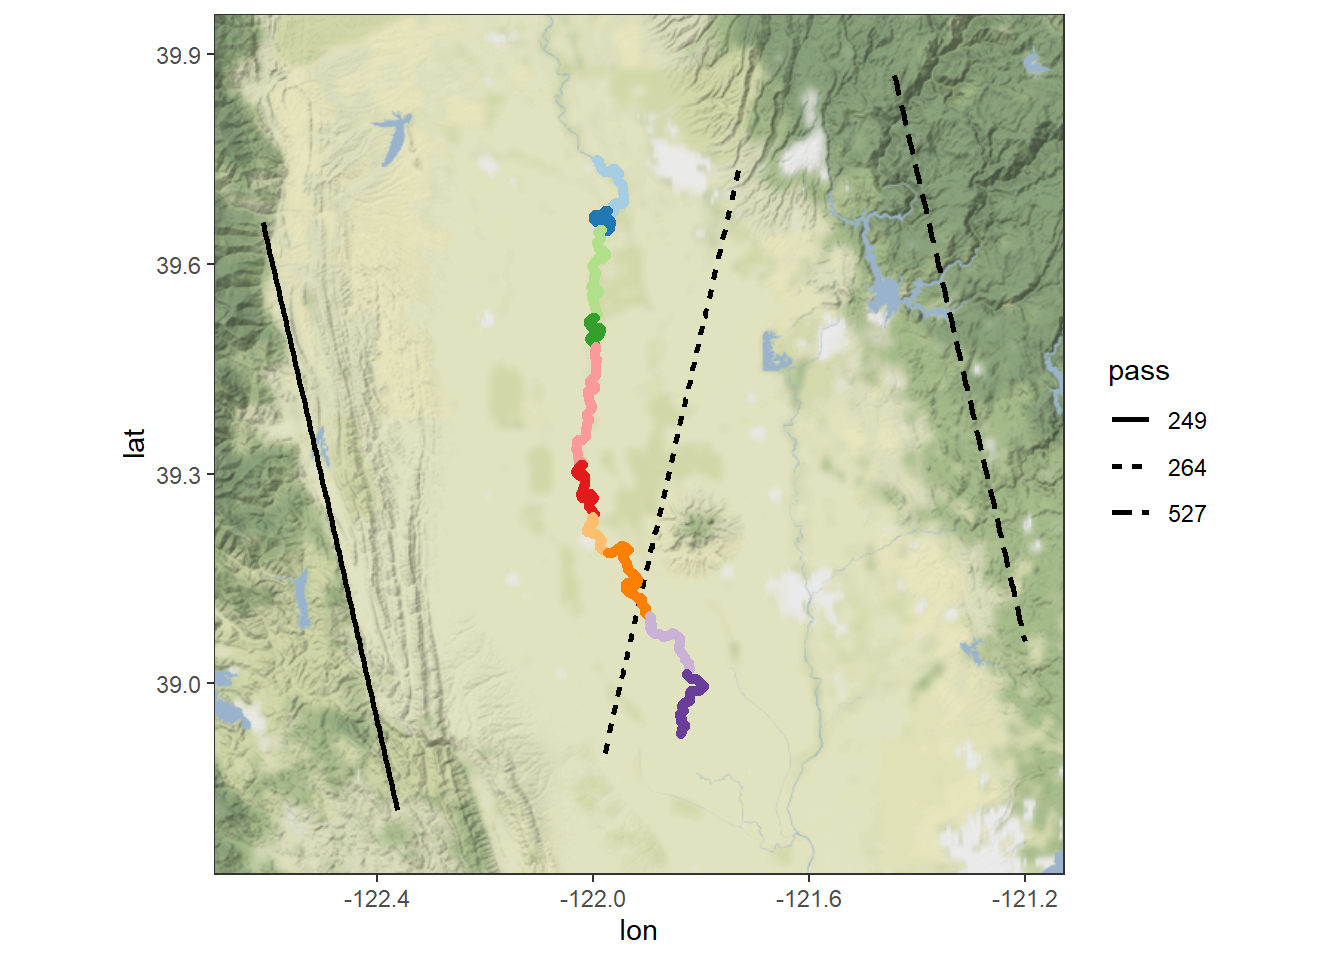
\includegraphics{_main_files/figure-latex/maps-1.pdf} 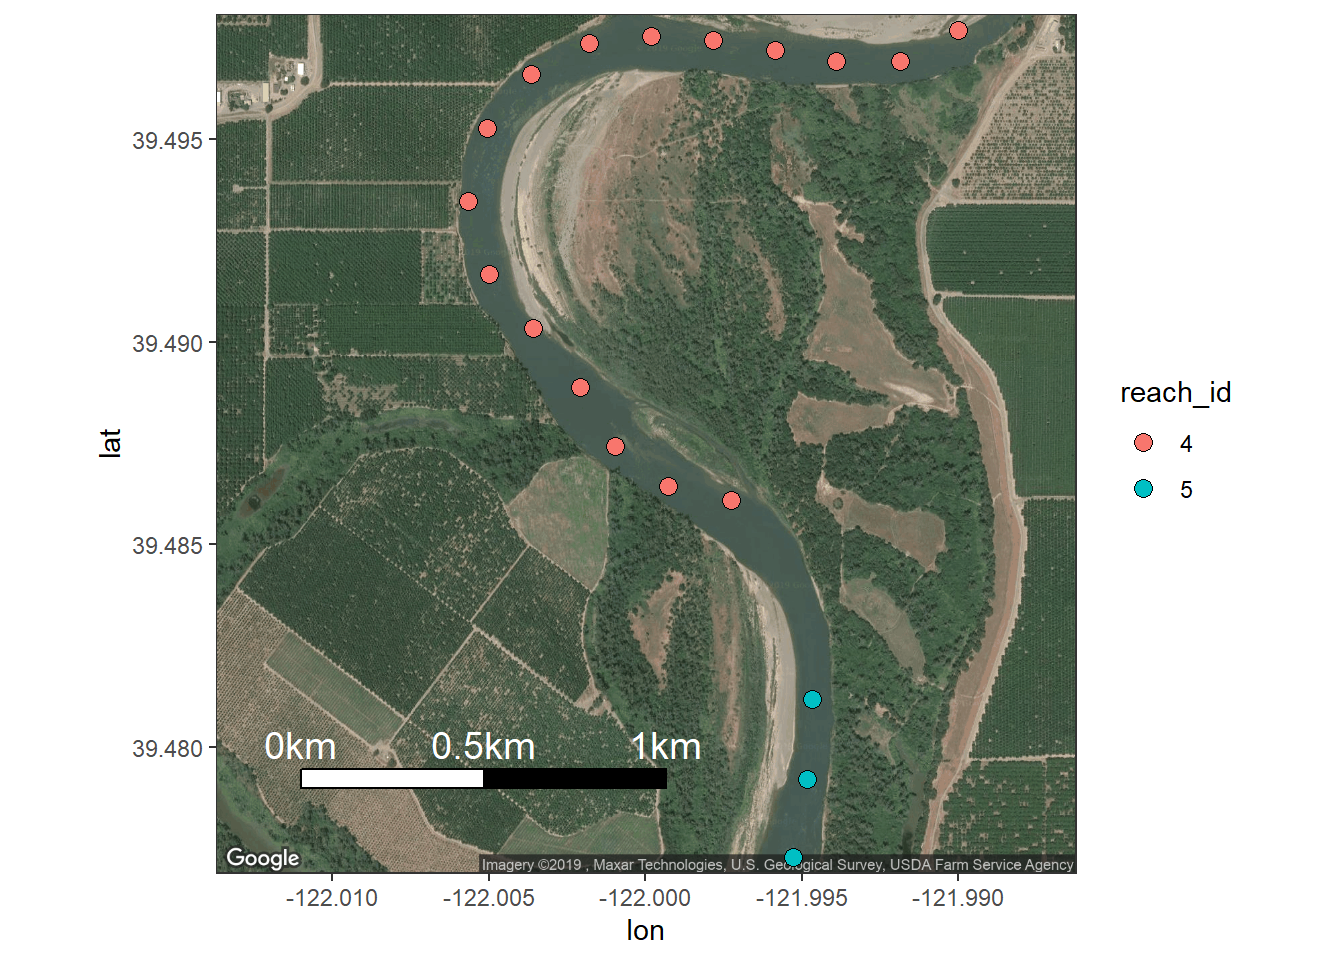
\includegraphics{_main_files/figure-latex/maps-2.pdf} 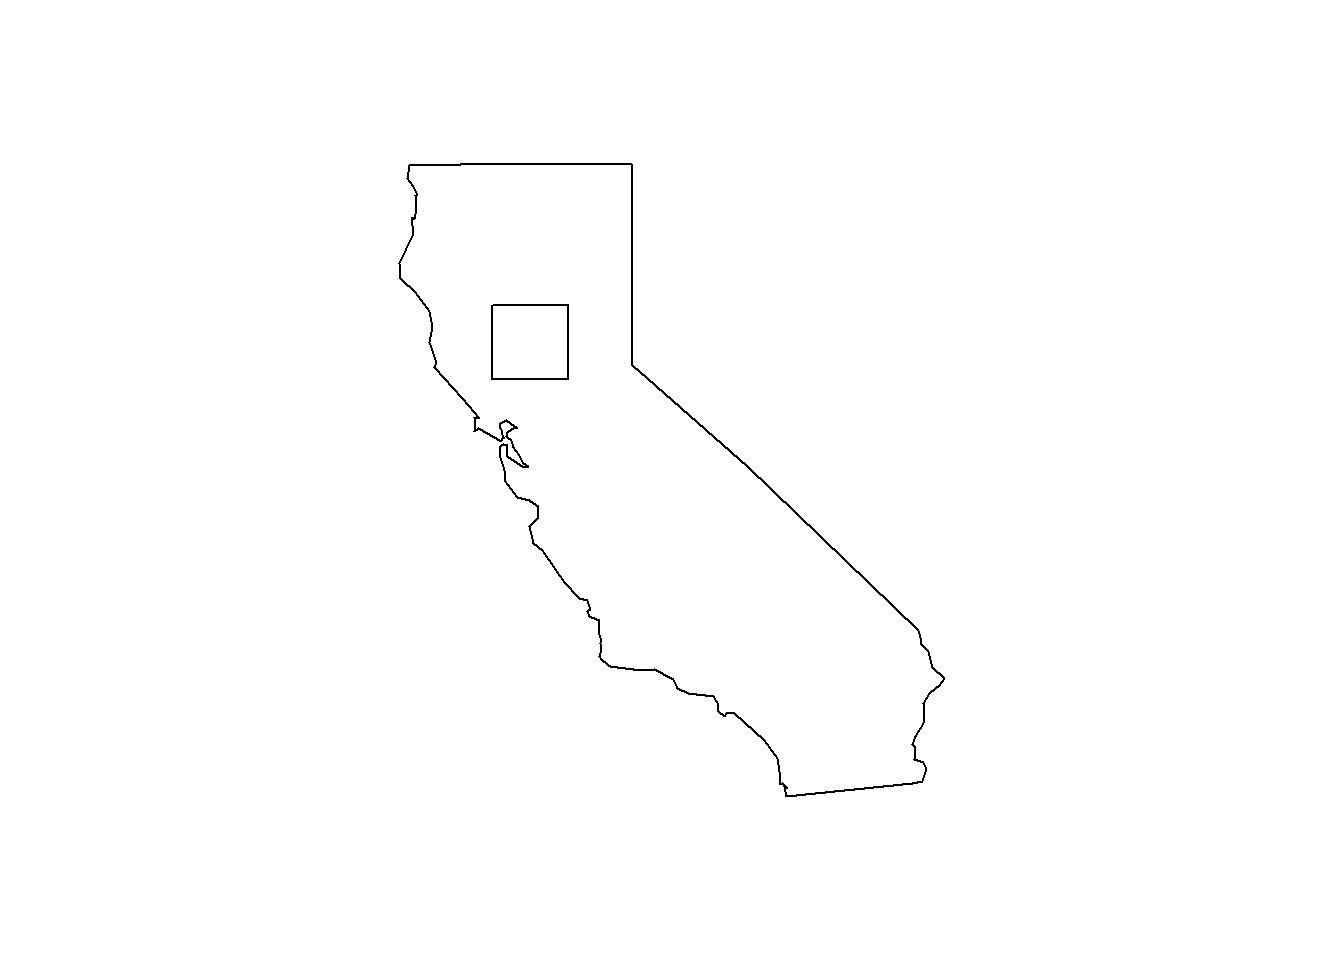
\includegraphics{_main_files/figure-latex/maps-3.pdf}

Validation of the simulated products requires a truth dataset; this was derived from a Global Digital Elevation Map (GDEM) model, produced from the ASTER NASA satellite. The GDEM was used to create a synthetic pixel cloud directly (in this case no precurser SLC was produced) and processed to create truth data for nodes and reaches in the study area. \#\#\#\#

Two sets of SWOT simulations were generated corresponding to more idealized and more realistic conceptions of land/water reflectance contrast and prior elevation information. The idealized case results in observation errors that arise from processes that are explicitly accounted for in the uncertainty estimation, whereas the realistic case includes potential un-modeled sources of error--namely phase unwrapping error and layover error, detailed below. This isolation of modeled and unmodeled error sources allowed for explicit validation of uncertainty models' representation of modeled phenomena as well as some indication of performance degradation due to unmodeled phenomena.

Phase information from the radar interferometer must be ``unwrapped'' in order to properly map radar data onto geospatial coordinates, and this requires a reference model of water surface elevation. The idealized case uses the GDEM truth as a reference model, whereas the realistic case uses a coarser-resolution Shuttle Radar Topography Mission (SRTM, \#\#\#\#REF) dataset for reference; SRTM will be used as the reference DEM for the operational SWOT mission. Layover errors arise when nearby land maps onto the same phase-range coordinates as water, resulting in biased heights for the affected water features (pixels, nodes, reaches). Layover was effectively turned off in the idealized simulations by setting land reflectance to be low (-100dB), whereas the realistic case used a higher land reflectance (-5dB). Both cases used a water reflectance of 10dB, and other simulation parameters were held constant across the two cases.

For each of the two simulation sets, 9 simulations were created using 3 passes and 3 cycles forced by observed discharge from February and March 2009 (Table \#\#\#\#). These simulations encompass a range of conditions affecting measurement error, including flow condition, number of pixels per node, and location of the water feature within the swath. Discharge over the simulated days ranged from 4662 to 36610 CFS, corresponding to the 6th and 96th percentiles of flow (Figure \#\#\#\#) as monitored by CA Dept of Water Resources (\url{http://cdec.water.ca.gov/dynamicapp/staMeta?station_id=HMC}). The three passes observe the study nodes and reaches across a wide range of positions within the swath, ranging from very near-swath (\textless10 km) in pass \#\#\#\# to very far swath (\textgreater60 km) in pass \#\#\#\#. The number of pixels per node ranged from \#\#\#\# to \#\#\#\# (Figure \#\#\#\#).

\begin{tabular}{r|r|r|r|r}
\hline
Date & Pass & n. nodes & flow (CFS) & flow pcntl.\\
\hline
2009-01-30 & 249 & 13131 & 4662 & 6.5\\
\hline
2009-01-31 & 264 & 7473 & 4595 & 5.9\\
\hline
2009-02-09 & 527 & 13143 & 4999 & 10.0\\
\hline
2009-02-20 & 249 & 13131 & 9224 & 67.3\\
\hline
2009-02-21 & 264 & 7473 & 7659 & 53.7\\
\hline
2009-03-02 & 527 & 13143 & 36610 & 95.7\\
\hline
2009-03-13 & 249 & 13131 & 6515 & 34.8\\
\hline
2009-03-14 & 264 & 7473 & 6370 & 32.3\\
\hline
2009-03-23 & 527 & 13143 & 6639 & 36.7\\
\hline
\end{tabular}

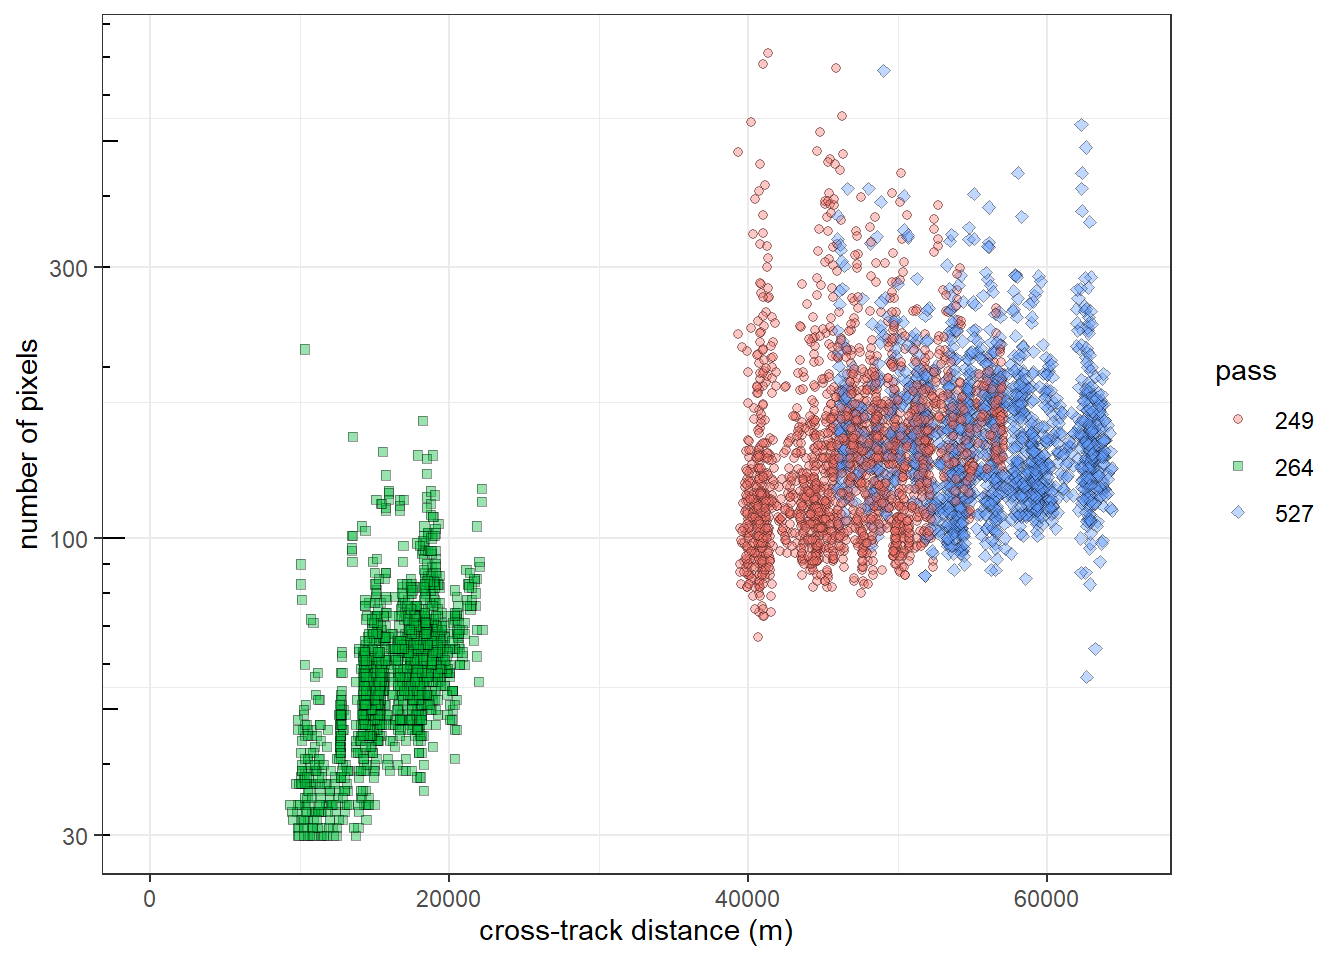
\includegraphics{_main_files/figure-latex/npx_xtk_gg-1.pdf}

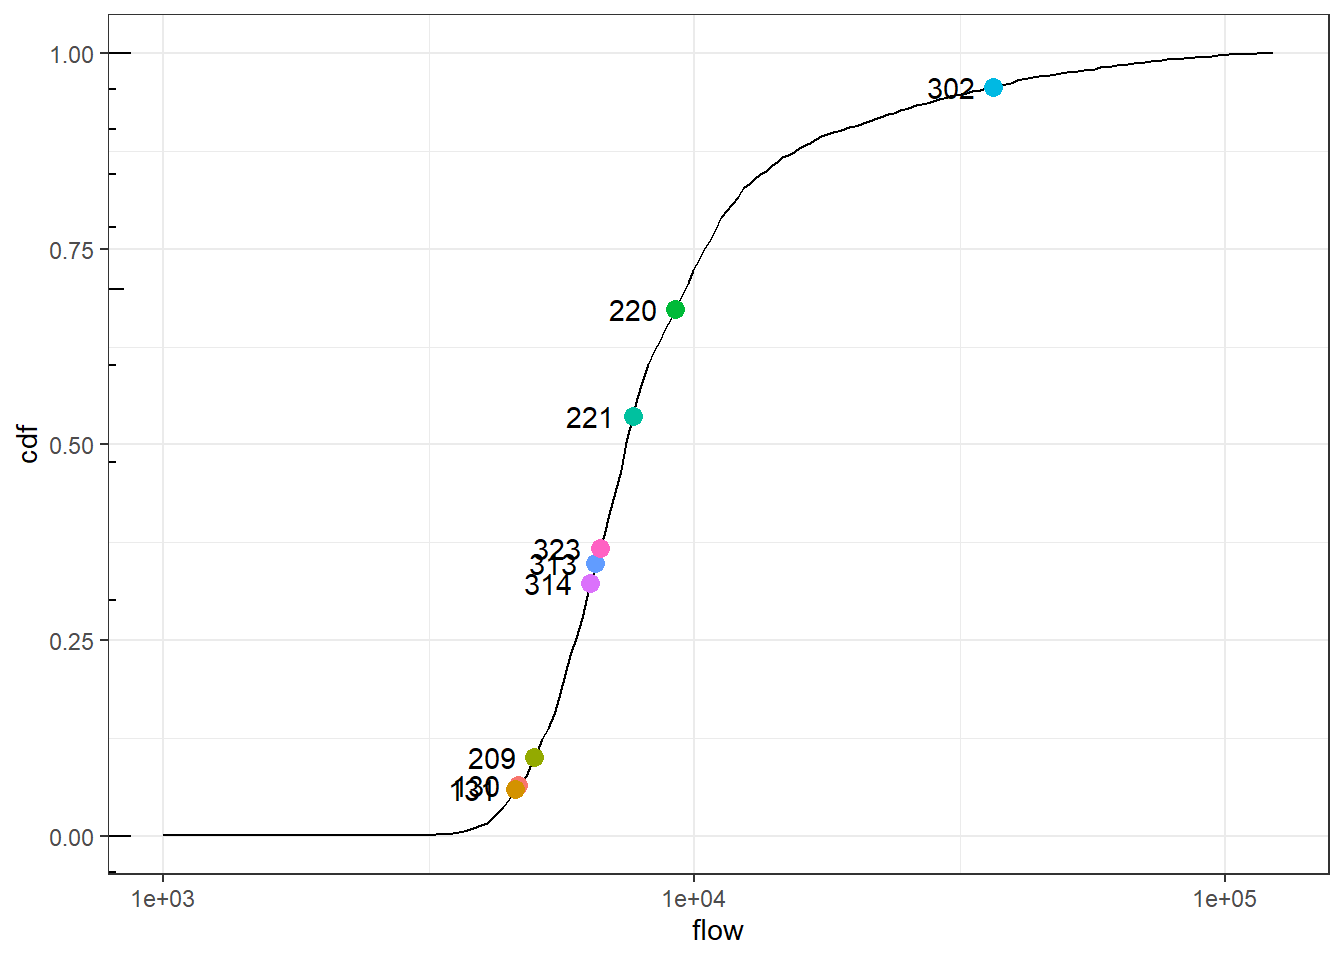
\includegraphics{_main_files/figure-latex/ecdf_gg-1.pdf}

\hypertarget{error-scaling}{%
\section{Error scaling}\label{error-scaling}}

The different SWOT observations are reported with estimates of \(1 \sigma\) uncertainty; the objective of uncertainty validation is to determine how accurately these uncertainty estimates match the behavior of empirical errors. In order to easily compare across a set of validation data with varying uncertainty estimates, we employ a simple transformation such that the mean and variance should be equal across all transformed validation data.

Consider an arbitrary measured variable (e.g.~node height, reach width, pixel latitude), denoted \(y_{st}\), where \(s\) indexes location (in \textbf{s}pace), and \(t\) indexes \textbf{t}ime. Because \(y\) is not precisely determined and has nonzero error, we can consider it a random variable. The corresponding true value, of which \(y\) is an estimate, is denoted \(y^*\). The error, \(\epsilon\), is defined as \(\epsilon = y - y^*\). Because \(\epsilon\) is a transformation of a random variable, it is itself a random variable. We denote the mean, variance, and standard deviation of \(\epsilon\) as \(\mu_\epsilon\), \(\sigma^2_\epsilon\), and \(\sigma_\epsilon\), respectively, and similarly for other random variables.

The objective of this study is to validate the quantification of uncertainty, where uncertainty is expressed as an estimate of \(\sigma_y\). We denote this estimate \(\hat{\sigma}_y\), to distinguish it from the true value \(\sigma_y\). We perform this validation over a potentially large number of locations \(s\) and times \(t\). The data for a given observed variable therefore consist of observations of \(y_{st}\) and \(\hat{\sigma}_{st}\); these are both provided in the SWOT river products.

In order to validate the estimates \(\hat{\sigma}_{st}\), we rely on analogous GDEM-derived synthetic data that give ``true'' values \(y^*_{st}\). Thus we can calculate a corresponding set of empirical errors \(\epsilon_{st}\) for every location and time in the dataset. Since \(\epsilon_{st} = y_{st} - y^*_{st}\), then if our uncertainty estimates are correct (\(\hat{\sigma}_{y_{st}} = \sigma_{y_{st}}\)), we obtain \(\sigma_{\epsilon_{st}} = \sigma_{y_{st}}= \hat{\sigma}_{y_{st}}\). A simple elementwise scaling, \(e_{st} \equiv \epsilon_{st} / \hat{\sigma}_{y_{st}}\) therefore has \(\sigma_{e_{st}} = 1\) for all \(s\) and \(t\). (Recall that for any random variable \(Y\) with mean \(\mu_Y\) and variance \(\sigma^2_Y\), a linear transformation of the form \(W = aY + b\) has mean \(\mu_W = a\mu_Y + b\) and variance \(a^2\sigma_Y^2\). This is true regardless of distribution.)

Thus scaled, the errors \(e_{st}\) can be compared across locations and times in order to validate the uncertainty estimates. A ``good'' model for \(\sigma_y\) will result in a set of \(e_{st}\) with empirical standard deviation that is close to 1. This observation leads directly to explicit tests for verifying the model responsible for producing \(\hat{\sigma}_{y_{st}}\).

\hypertarget{results}{%
\chapter{Results}\label{results}}

How well do uncertainty models characterize empirical errrors from simulated SWOT data? The answer depends on the variable measured, the data product (node or reach), the simulation characteristics, and the particularities of aggregation. The validation results are presented here separately for different variables and data products.

\hypertarget{node-results}{%
\section{Node Results}\label{node-results}}

Scaled node-level errors varied in behavior across the different simulations and variables. Height error RMSE was generally less than 1.3 for the realistic simulations--with most of this coming from bias--and less than 1.1 for the idealized simulations--which had negligible bias. Scaled width errors were more variable, with RMSE as high as 5x the model-predicted RMSE in the simple aggregation, 2x the predicted RMSE using composite aggregation, and 1.5x the predicted RMSE using water-fraction aggregation. The simulation parameters--idealized versus realistic--had only a minor effect on width error statistics.

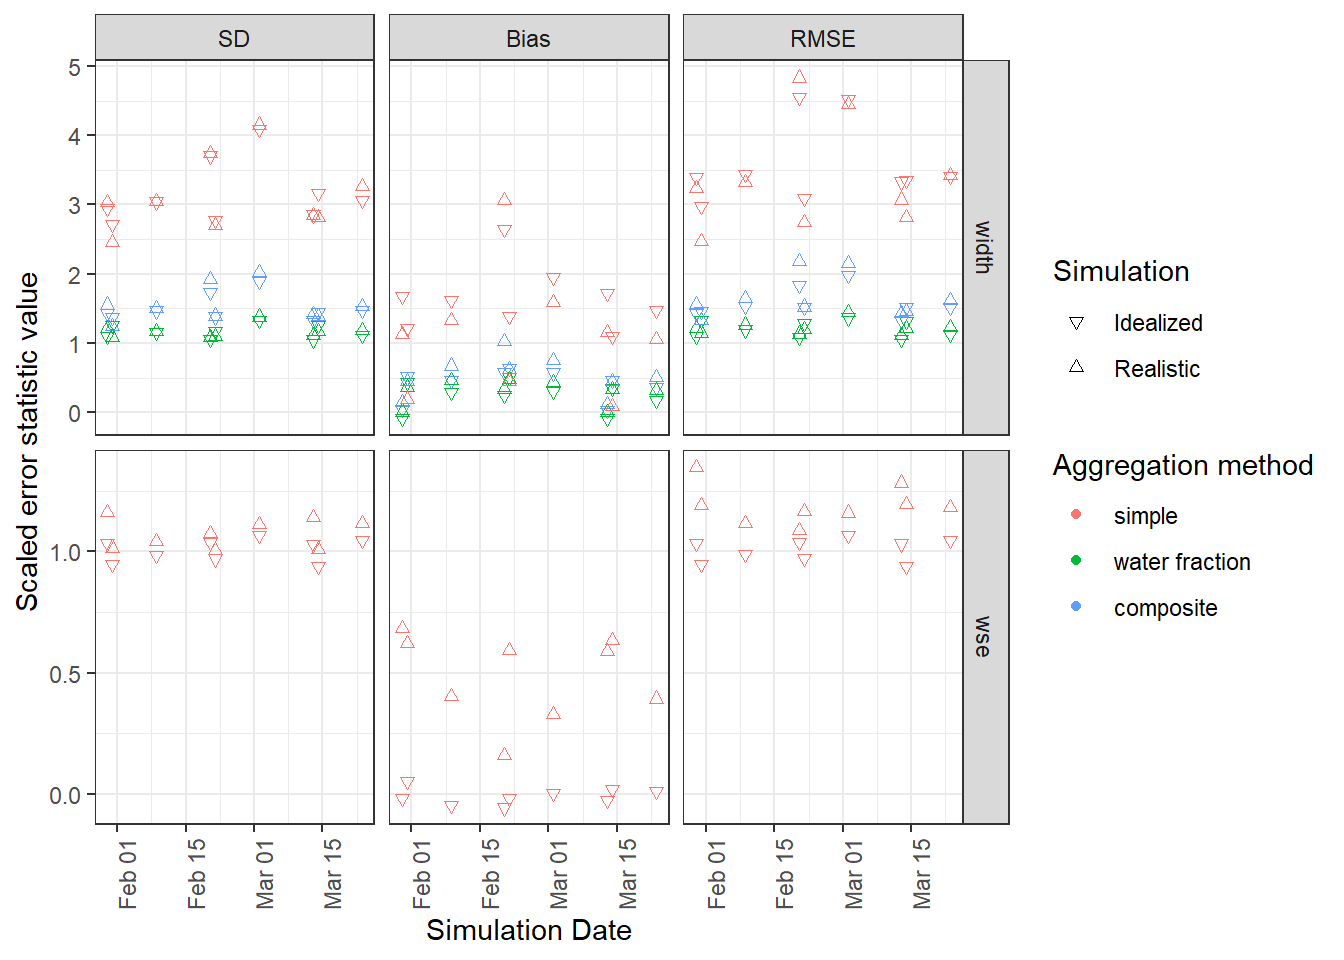
\includegraphics{_main_files/figure-latex/nodesdplot-1.pdf} 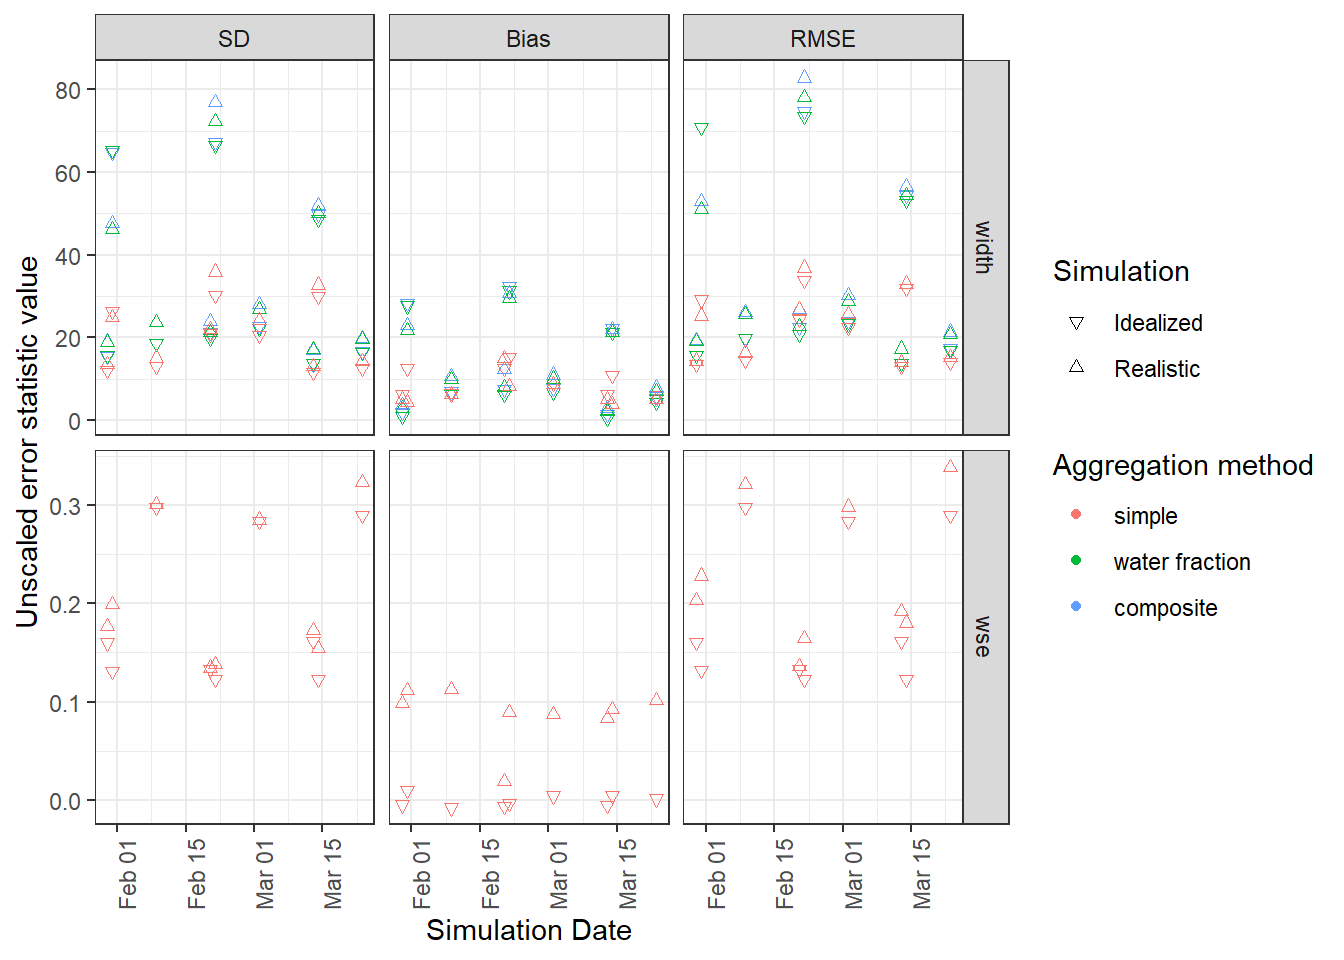
\includegraphics{_main_files/figure-latex/nodesdplot-2.pdf}

Normal quantile-quantile (QQ) plots (Fig. \#\#\#\#) compare the emprical scaled errors to the theoretical \(N(0, 1)\) distribution (solid black line) for ``water fraction'' aggregtion and idealized simulation parameters. This distinguishes characteristics of the empirical error distribution including bias (vertical offset from 1:1 line), standard deviation (slope of points), and departures from normality, for instance heavy tails. Based on Fig. \#\#\#\#, the uncertainty model for height adequately characterized uncertainty across all simulation dates and for all parts of the distribution, with approximately standard normal scaled errors. In contrast, scaled width errors exhibit heavy-tailed distributions, especially at the upper tail, corresponding to errors that are much higher than would be expected if the errors were normally distributed. Despite this behavior in the tails, the middle of the scaled width error distribution was more well-behaved, with small but non-negligible bias depending on the simulation date.

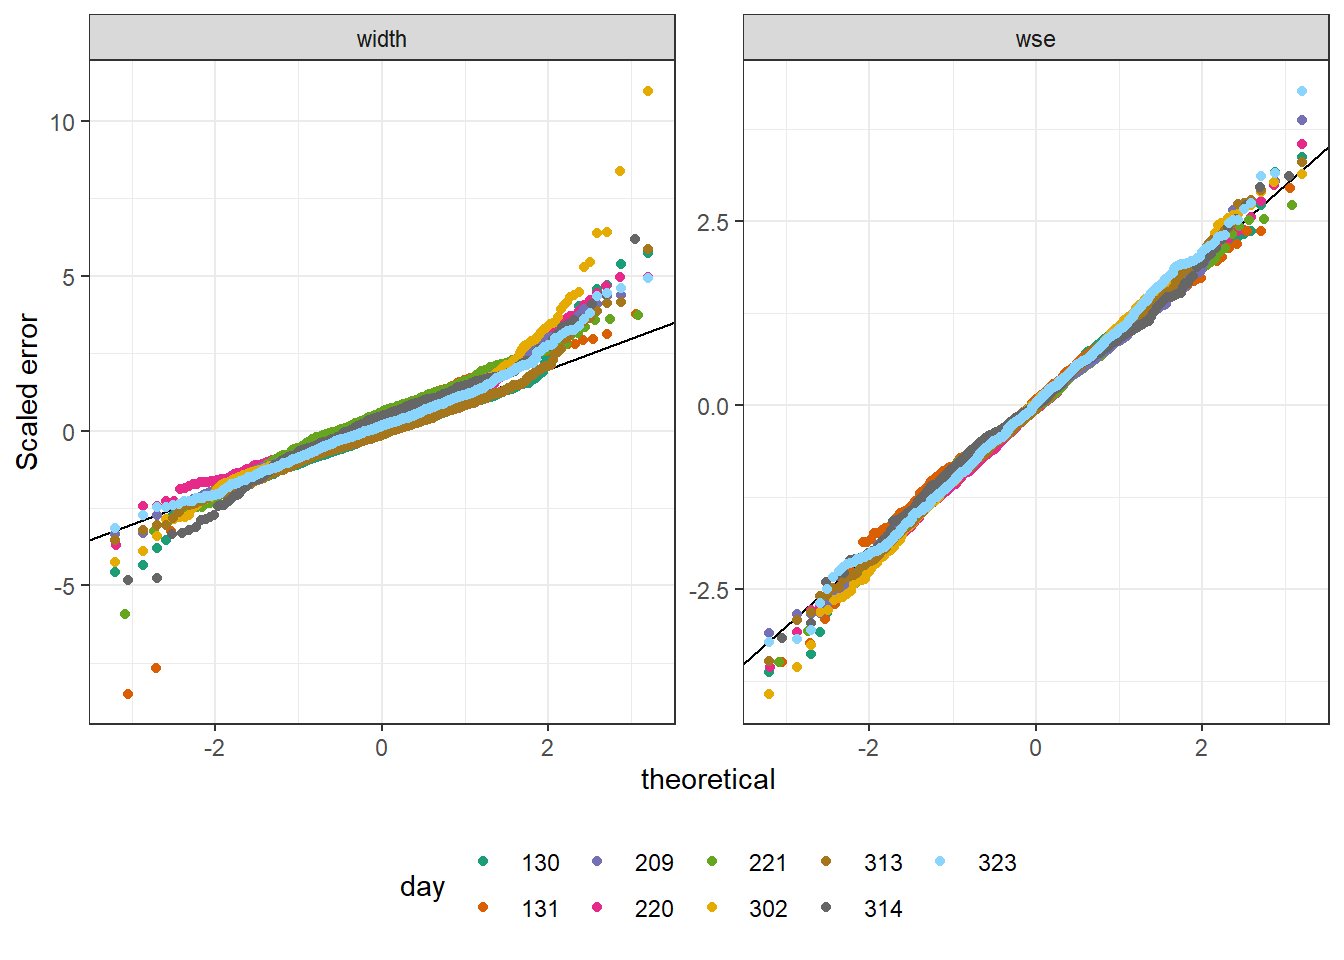
\includegraphics{_main_files/figure-latex/qqplot_byday-1.pdf}

In aggregate across all simulation days, distributions of scaled node height and width errors exhibit broadly the same characteristics as the same distributions for individual simulation days, but differ in severity by depending on the simulation parameters (Fig. \#\#\#\#). Width errors were closest in distribution to standard normal for the ``water fraction'' aggregation method, while using the composite method resulted in a heavier right-skew, and the simple mehtod had both a severely large upper tail as well as higher variance throughout the distribution (Fig. \#\#\#\#a). Height error distributions were unaffected by aggregation method, but adding simulation noise resulted in significant bias and slightly larger variance (Fig. \#\#\#\#b.

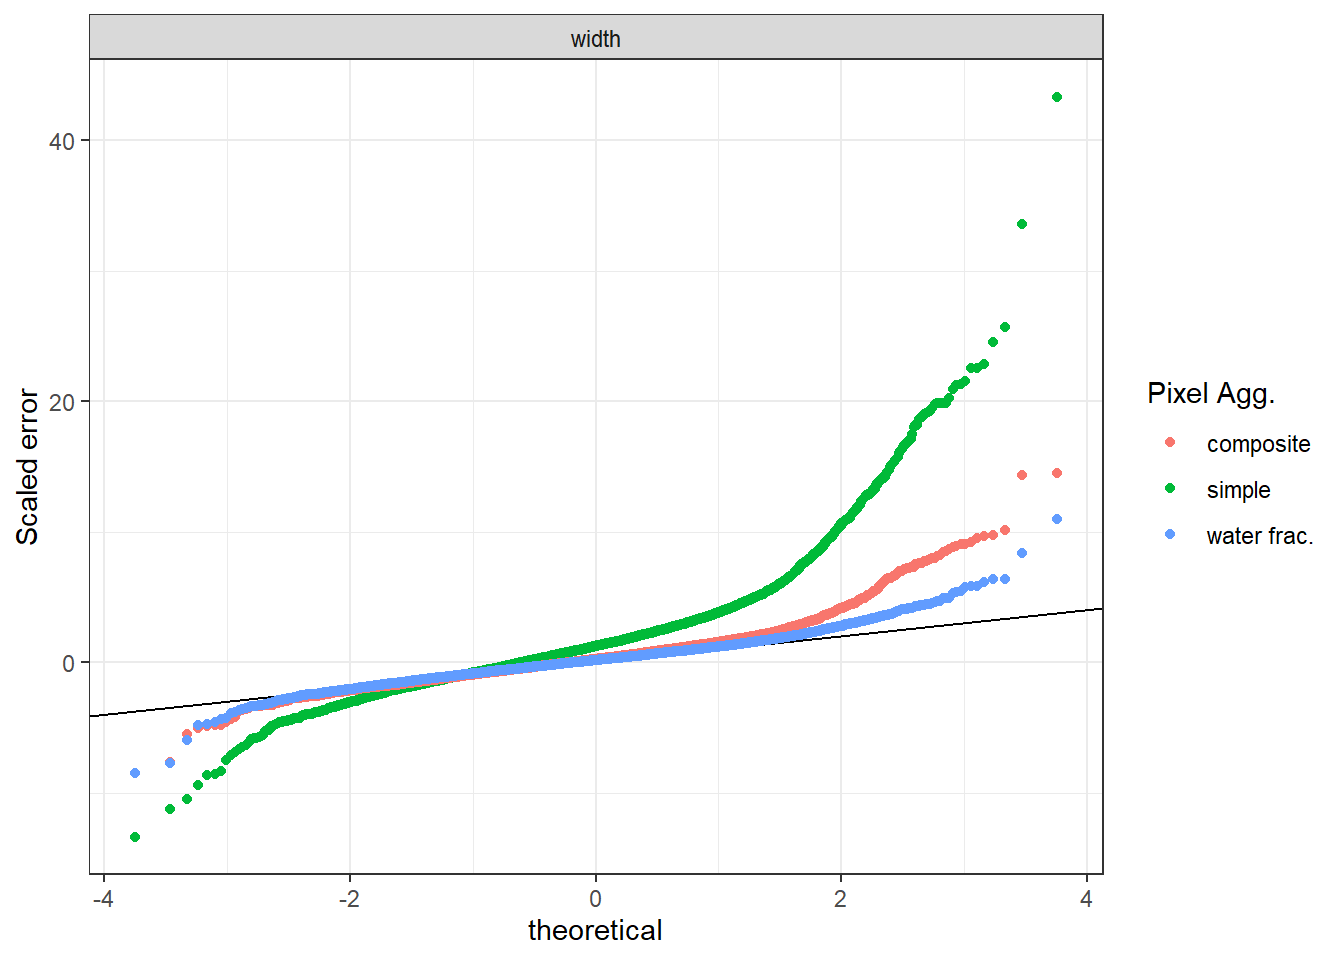
\includegraphics{_main_files/figure-latex/qqplot_bycondition-1.pdf} 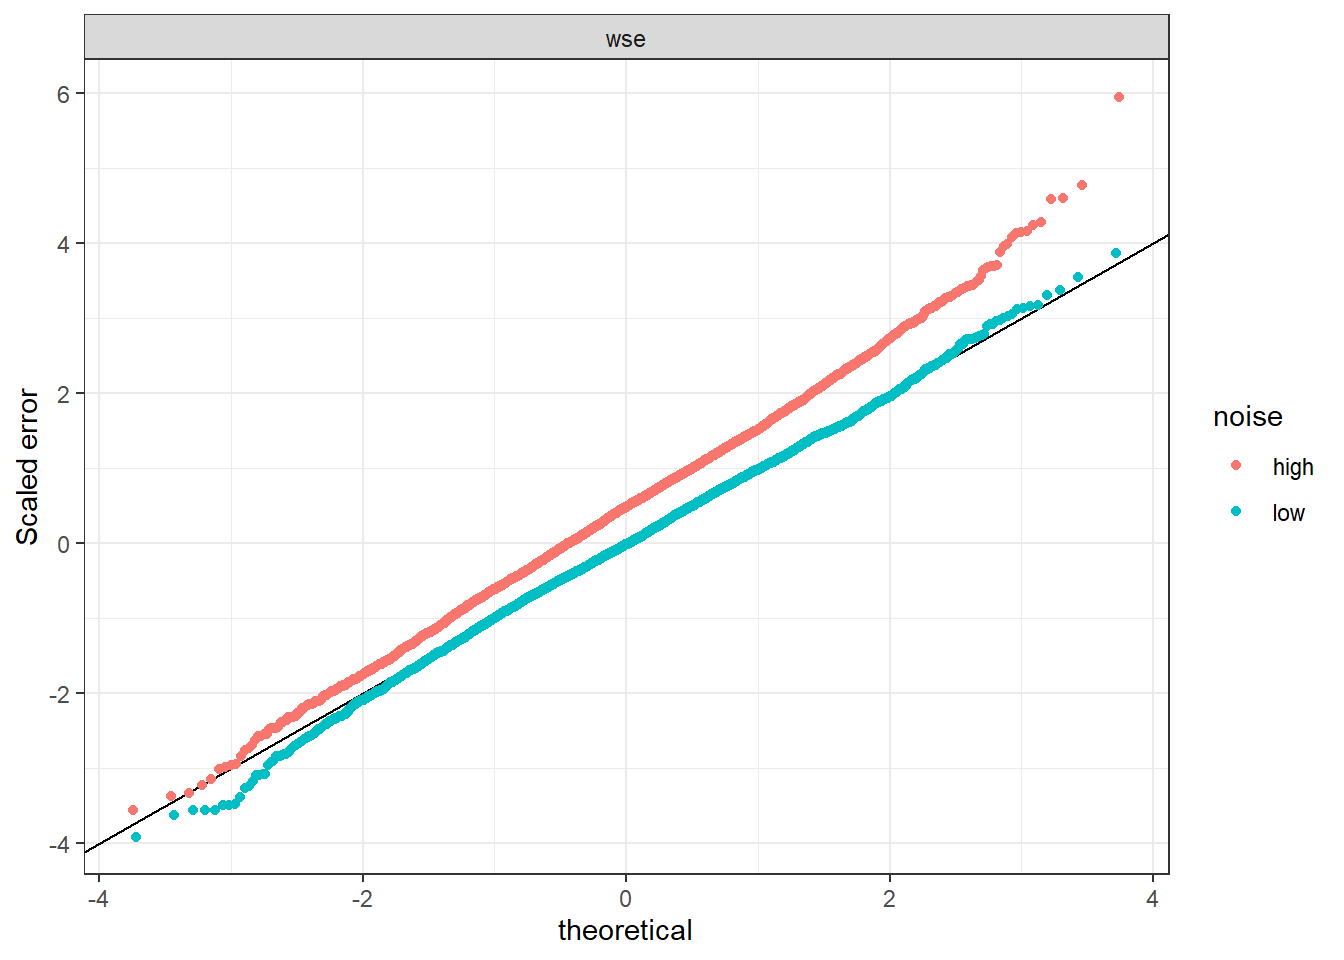
\includegraphics{_main_files/figure-latex/qqplot_bycondition-2.pdf}

\hypertarget{factors-affecting-node-level-errors-and-uncertainty}{%
\subsection{Factors affecting node-level errors and uncertainty}\label{factors-affecting-node-level-errors-and-uncertainty}}

Node-level height errors vary as a function of the number of pixels per node and the distance from the node to the ground-track of the satellite. These effects are not independent, since pixel size is larger closer to the ground track, resulting in fewer pixels for a given node area. A node with fewer pixels will have less ability to average out the independent noise per pixel, resulting in larger node-level errors. Pixel height errors also increase farther from the ground-track, as height becomes increasingly sensitive to changes in interferometric phase with increasing cross-track distance. These two phenomena--pixel size and height-phase sensitivity--result in a U-shaped relationship between estimated height uncertainty and cross-track distance (Fig. \#\#\#\#d). Both of these effects are well characterized in the height uncertainty model, resulting in scaled errors lying generally between -2 and 2, as expected given unit standard deviation.

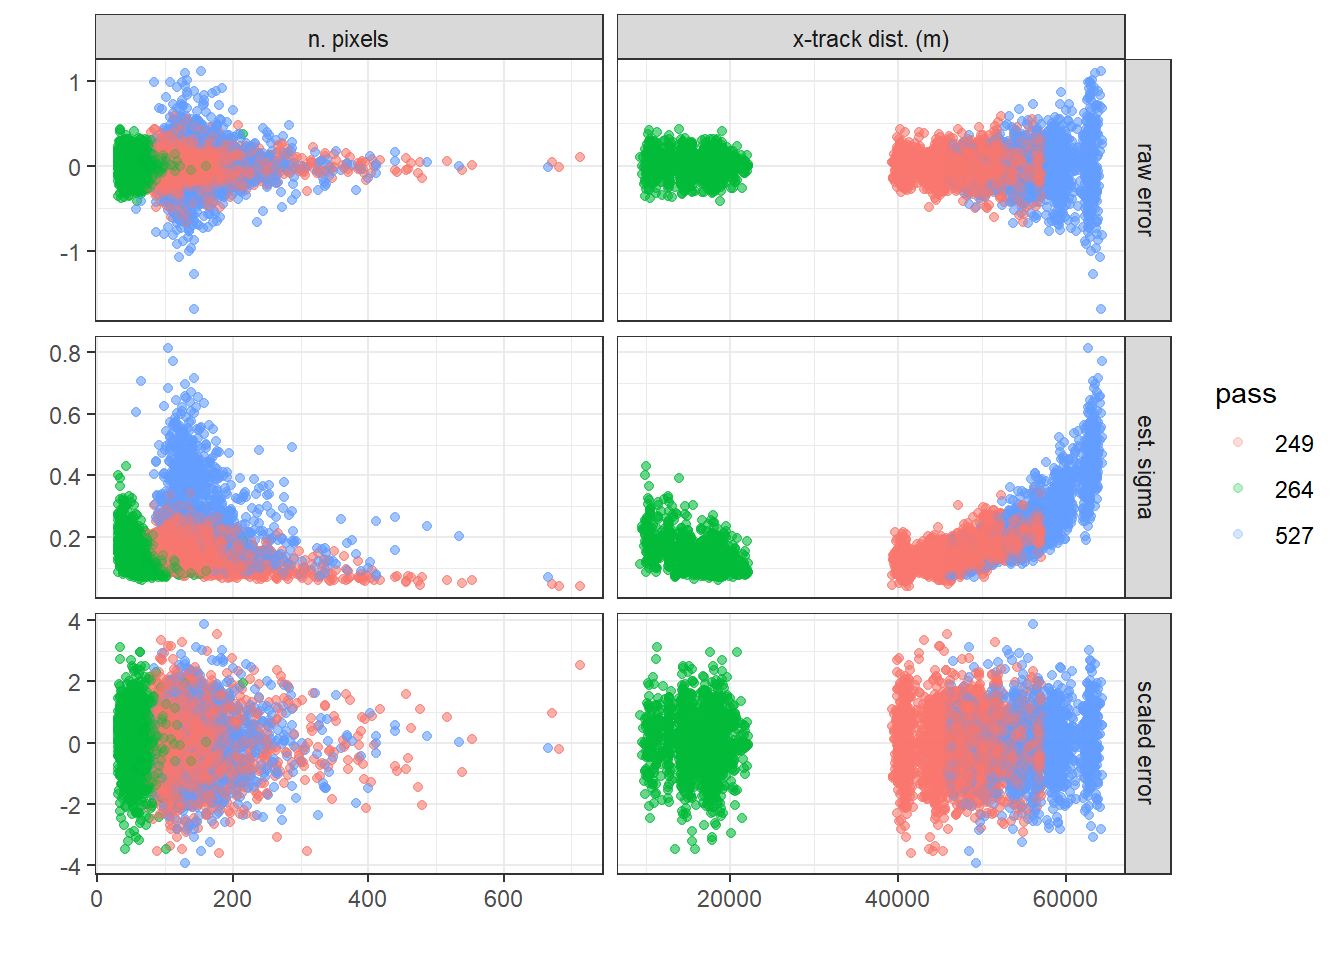
\includegraphics{_main_files/figure-latex/wse_scatter-1.pdf}

Width errors are also affected by pixel size, but are not otherwise affected by cross-track distance, resulting in the error and uncertainty profile shown in Fig. \#\#\#\#a-d.~While the scaled width errors are not as well-behaved as the height errors and exceed 10 or 20 times the estimated \(1\sigma\) uncertainty, they exhibit no discernable patterns when plotted against pixel count or cross-track distance, suggesting that these effects are well characterized by the uncertainty model.

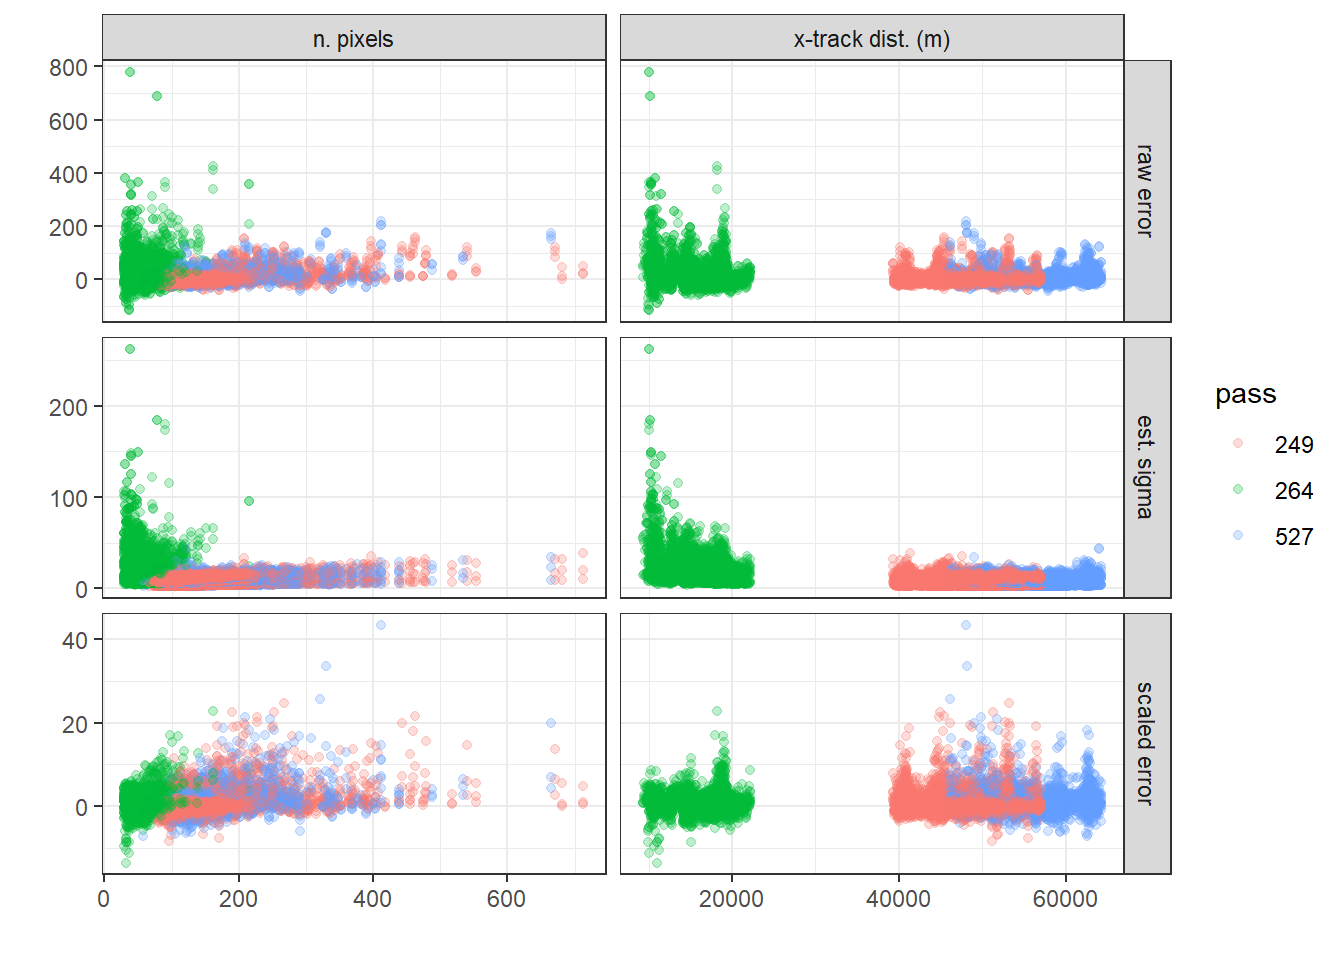
\includegraphics{_main_files/figure-latex/width_scatter-1.pdf}

\hypertarget{reach-results}{%
\section{Reach results}\label{reach-results}}

Scaled reach-level errors for height and slope measurements (Fig. \#\#\#\#, top row) were apparently unbiased and fell generally between -2 and 2 in the idealized simulations, reflecting well-characterized uncertainties. As at the node level, corresponding width errors were less well-behaved, reaching as much as 10 times the \(1\sigma\) uncertainty estimate. The magnitude of scaled width errors were larger on average than at the node scale, resulting from violations of underlying assumptions (zero bias, independence) when aggregating node to reach uncertainty.

In the ``realistic'' simulations, introducing simulation noise primarily affected height errors--biasing many simulations' reach errors--but also had non-negligible effects on slope and width errors (Fig. \#\#\#\#, bottom row). Slope errors were larger in magnitude in some reaches--notably reaches 6 and 8. Width errors varied more sporadically, increasing or decreasing depending on the simulation day and reach.

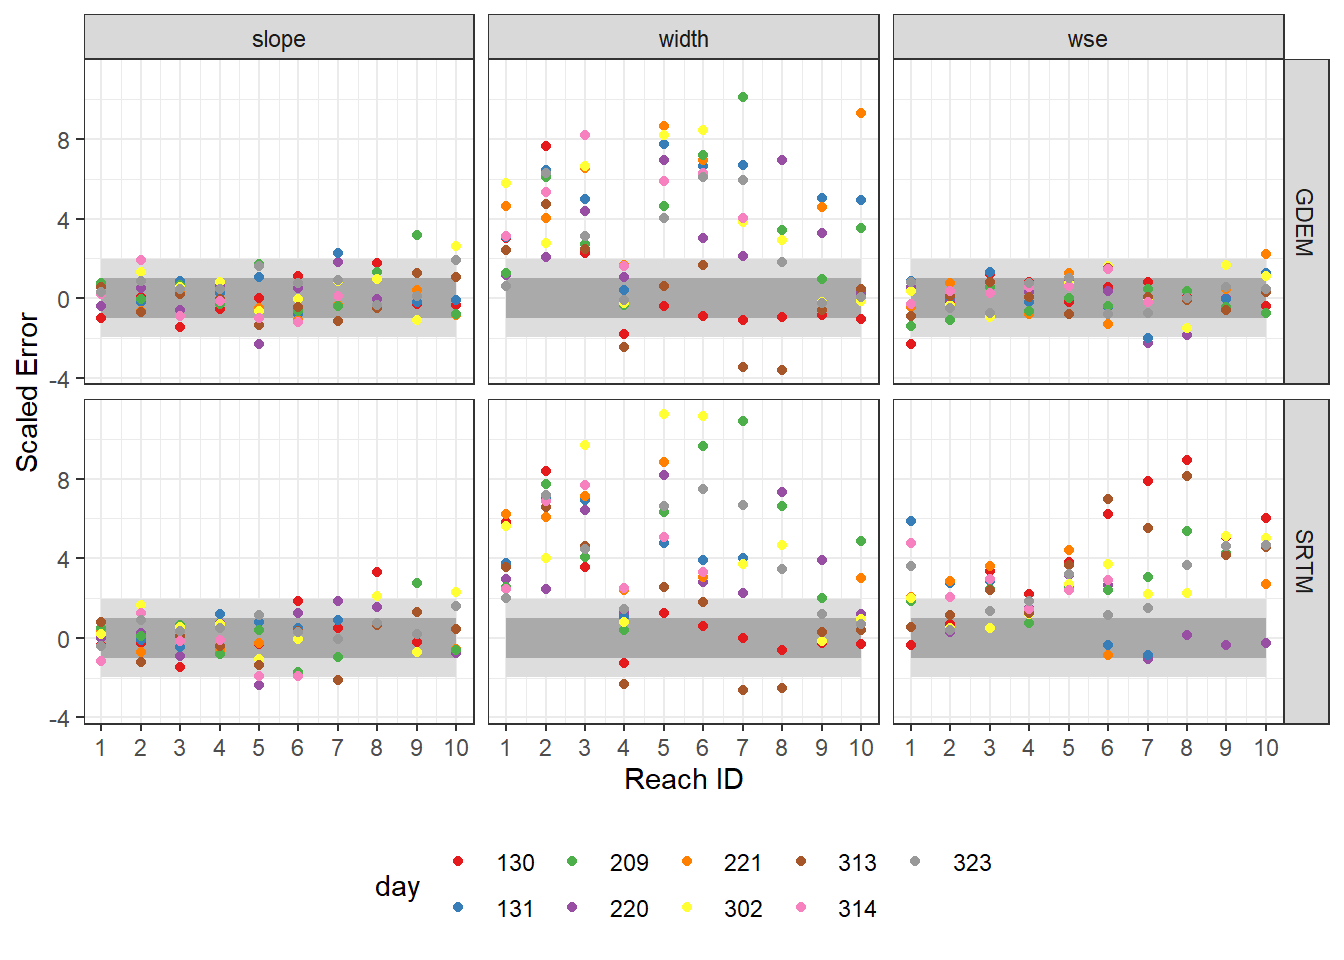
\includegraphics{_main_files/figure-latex/reach_scatter-1.pdf}

\hypertarget{large-width-errors}{%
\section{Large width errors}\label{large-width-errors}}

Both the node-scale and reach-scale errors have right-skewed distributions, resulting from relatively infrequent sections of river having outsized influence on the aggregated errors. These errors result mainly from three distinct phenomena: complex channel geometry, spurious contiguity of water pixels, and narrow channels relative to pixel size. These are described in detail in the following text, and illustrated in Figure \#\#\#\#.

\begin{enumerate}
\def\labelenumi{\arabic{enumi}.}
\tightlist
\item
  Complex channel geometry that cannot be resolved, either due to pixel size or regularization in slant plane (Fig. \#\#\#\#a)
\item
  Sections of water that are contiguous in the PIXC slant plane but not in the validation slant plane, resulting in pixels for a given area of water being assigned to nodes in the PIXC that are not assigned to the node in the GDEM PIXC. (Fig. \#\#\#\#b)
\item
  Stretches of river that are narrow in comparison to the pixel size, with an apparent positive bias in water fraction estimates for water-edge pixels. (Fig. \#\#\#\#c).
\end{enumerate}

\hypertarget{illustration-of-nodes-with-large-errors}{%
\subsection{Illustration of nodes with large errors}\label{illustration-of-nodes-with-large-errors}}

While pixel-level data do not have a 1:1 correspondence between simulated and validation data and thus cannot be compared directly, visual juxtaposition of pixel data illustrative of phenomena that lead to large width errors. These phenomena include:

\begin{enumerate}
\def\labelenumi{\arabic{enumi}.}
\tightlist
\item
  Complex channel geometry that cannot be resolved, either due to pixel size or regularization in slant plane (Fig. \#\#\#\#a)
\item
  Sections of water that are contiguous in the PIXC slant plane but not in the validation slant plane, resulting in pixels for a given area of water being assigned to nodes in the PIXC that are not assigned to the node in the GDEM PIXC. (Fig. \#\#\#\#b)
\item
  Stretches of river that are narrow in comparison to the pixel size, with an apparent positive bias in water fraction estimates for water-edge pixels. (Fig. \#\#\#\#c)
\end{enumerate}

All 3 of these phenomena are spatially correlated--nodes that experience them tend to occur in clusters. Thus the resulting errors at the reach scale are larger in magnitude, since node-to-reach uncertainty accumulation assumes that errors are spatially independent.

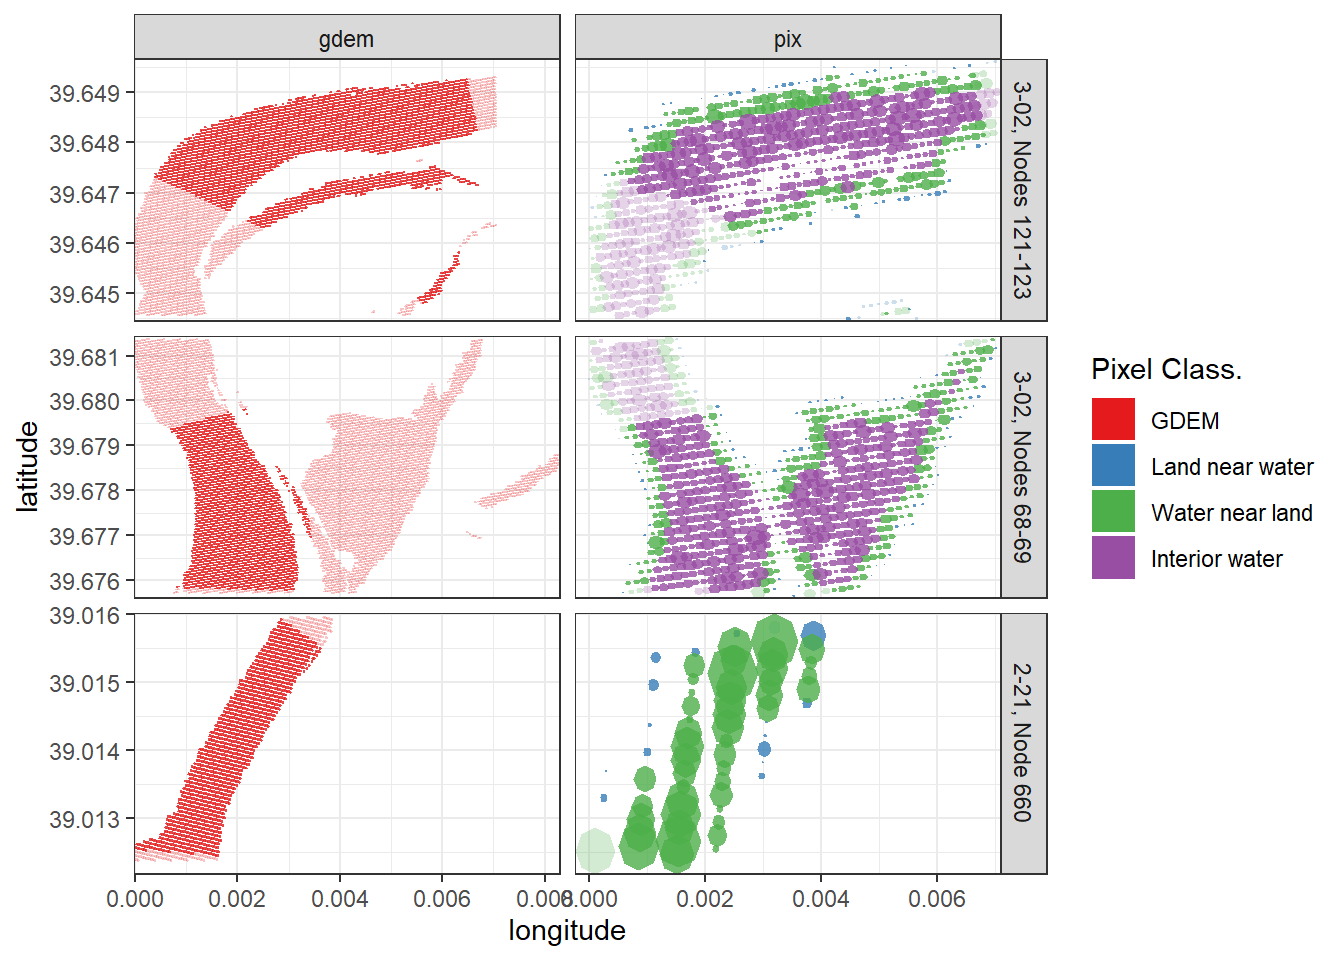
\includegraphics{_main_files/figure-latex/pix_maps-1.pdf}

\hypertarget{discussion}{%
\chapter{Discussion}\label{discussion}}

\hypertarget{random-systematic-error-partitioning}{%
\subsection{Random-systematic error partitioning}\label{random-systematic-error-partitioning}}

Uncertainty can be parsed into two components--bias and variance, corresponding to ``systematic'' and ``random'' errors. Strictly speaking, if \(\sigma_y\) is defined to be a standard deviation (square root of variance), then it does not include bias, and therefore ignores a potentially large component of uncertainty. Adjusting \(\hat{\sigma}_y\) cannot remove this bias, but it can account for it by ``lumping it in'' to the variance. This choice of whether or not to account for bias leads to two separate sets of uncertainty validation--with and without bias-adjusting the scaled errors. Since the uncertainty estimates are produced using a method that explicitly assumes zero bias, it makes sense to validate these estimates without including bias. On the other hand, real-world errors will include both random and systematic components, and a true assessment of uncertainty should somehow measure how well uncertainty estimates account for the full error distribution--including bias.

\hypertarget{particularities-of-sacramento-river}{%
\subsection{Particularities of Sacramento River}\label{particularities-of-sacramento-river}}

The selection of the Sacramento River for this validation study was a choice of convenience, since the authors had access to a calibrated numerical model to faciliatate simulation of 2-dimensional water height

\hypertarget{refs}{}
\leavevmode\hypertarget{ref-swot2018calval}{}%
?? 2018. ``SWOT Calibration / Validation Plan.'' Jet Propulsion Laboratory, California Institute of Technology; NASA.

\leavevmode\hypertarget{ref-altenau2017}{}%
Altenau, Elizabeth H, Tamlin M Pavelsky, Delwyn Moller, Christine Lion, Lincoln H Pitcher, George H Allen, Paul D Bates, Stéphane Calmant, Michael Durand, and Laurence C Smith. 2017. ``AirSWOT Measurements of River Water Surface Elevation and Slope: Tanana River, Ak.'' \emph{Geophysical Research Letters} 44 (1): 181--89.

\leavevmode\hypertarget{ref-andreadis2018}{}%
Andreadis, Konstantinos M. 2018. ``Data Assimilation and River Hydrodynamic Modeling over Large Scales.'' In \emph{Global Flood Hazard: Applications in Modeling, Mapping, and Forecasting}, 229--37. Hoboken, NJ, USA: Wiley Online Library.

\leavevmode\hypertarget{ref-durand2016}{}%
Durand, Michael, CJ Gleason, Pierre-André Garambois, David Bjerklie, LC Smith, Hélène Roux, Ernesto Rodriguez, et al. 2016. ``An Intercomparison of Remote Sensing River Discharge Estimation Algorithms from Measurements of River Height, Width, and Slope.'' \emph{Water Resources Research} 52 (6): 4527--49.

\leavevmode\hypertarget{ref-durand2014}{}%
Durand, Michael, Jeffrey Neal, Ernesto Rodrı́guez, Konstantinos M Andreadis, Laurence C Smith, and Yeosang Yoon. 2014. ``Estimating Reach-Averaged Discharge for the River Severn from Measurements of River Water Surface Elevation and Slope.'' \emph{Journal of Hydrology} 511: 92--104.

\leavevmode\hypertarget{ref-fu2012swot}{}%
Fu, Lee-Lueng, Douglas Alsdorf, Rosemary Morrow, Ernesto Rodriguez, and Nelly Mognard. 2012. ``SWOT: The Surface Water and Ocean Topography Mission: Wide-Swath Altimetric Elevation on Earth.'' Jet Propulsion Laboratory, California Institute of Technology; NASA.

\leavevmode\hypertarget{ref-gleason2017}{}%
Gleason, CJ, PA Garambois, and MT Durand. 2017. ``Water, Satellites, and Mass Conservation: Tracking River Flows from Space.'' \emph{Eos, Transactions American Geophysical Union} 98.

\leavevmode\hypertarget{ref-oubanas2018}{}%
Oubanas, Hind, Igor Gejadze, Pierre-Olivier Malaterre, and Franck Mercier. 2018. ``River Discharge Estimation from Synthetic Swot-Type Observations Using Variational Data Assimilation and the Full Saint-Venant Hydraulic Model.'' \emph{Journal of Hydrology} 559: 638--47.

\leavevmode\hypertarget{ref-pitcher2019}{}%
Pitcher, Lincoln H, Tamlin M Pavelsky, Laurence C Smith, Delwyn K Moller, Elizabeth H Altenau, George H Allen, Christine Lion, et al. 2019. ``AirSWOT Insar Mapping of Surface Water Elevations and Hydraulic Gradients Across the Yukon Flats Basin, Alaska.'' \emph{Water Resources Research} 55 (2): 937--53.

\leavevmode\hypertarget{ref-tuozzolo2019}{}%
Tuozzolo, S, G Lind, B Overstreet, J Mangano, M Fonstad, M Hagemann, RPM Frasson, et al. 2019. ``Estimating River Discharge with Swath Altimetry: A Proof of Concept Using Airswot Observations.'' \emph{Geophysical Research Letters} 46 (3): 1459--66.


\end{document}
